\section{Results}
In Figure \ref{aha-fig:graphsize} we present the size of the abstract graphs relative to the size of the original graphs which featured an average 4469 nodes and 16420 edges. 
We look at the effect of increasing the amount of soft obstacles (SO) from 0\% (the original test maps with only one traversable terrain) to 50\%.
We also contrast high and low quality abstractions (denoted HQ and LQ) on a range of cluster sizes $\lbrace 10, 15, 20 \rbrace$ (denoted CS10, CS15 and CS20).
\begin{figure}[htbp]
	\vspace{-12pt}
       \caption{\small{\emph{Percentage of nodes and edges in abstract graph with respect to original graph. }}}
       \begin{center}
                       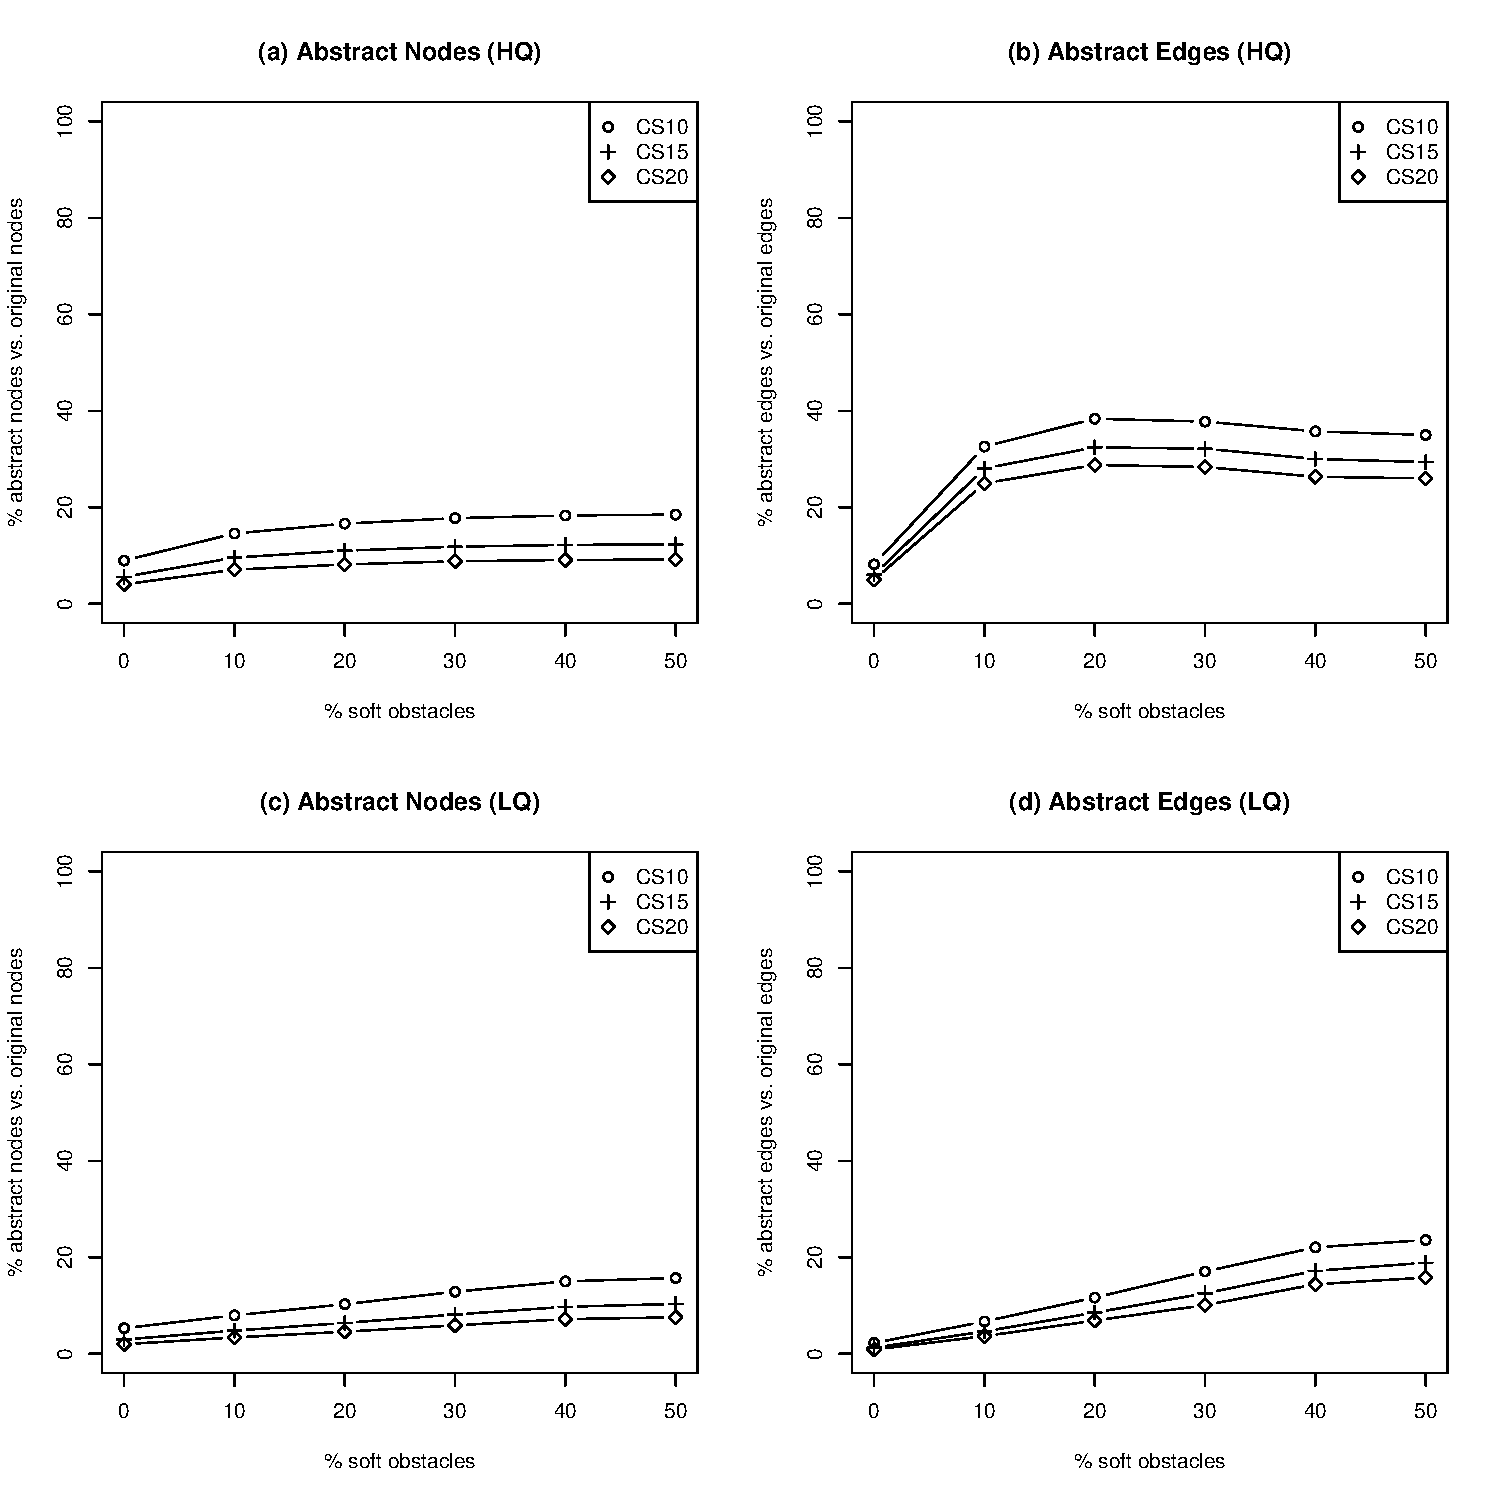
\includegraphics[scale=0.35, trim = 20mm 14mm 20mm 5mm]{diagrams/graphsize.pdf}
       \end{center}
       \label{aha-fig:graphsize}
	\vspace{-4pt}
\end{figure}
\par \indent
The first thing to notice is that in all cases the abstract graph is only a fraction the size of the original graph.
As expected, larger clusters generate smaller graphs; the smallest abstractions are observed on the SO 0\% problem set using CS20. 
In this case, using a HQ abstraction results in 4.0\% the number of nodes found in the original graph and 5.0\% edges. 
LQ abstractions fare even better featuring just 2.0\% as many nodes and 0.9\% edges.
\par \indent
The total space complexity associated with storing a graph is given by the total amount of space required to store both nodes and edges.
If we assume each non-abstract node and edge require one byte of memory to store, then our smallest abstract graph, which contains 2 annotations per edge (capability and clearance, together requiring 1 additional byte), will have a space complexity 8.7\% the size of the original graph using a HQ abstraction and just 1.8\% using an LQ abstraction.
Similarly, the largest HQ graph, which occurs for CS10 on SO 20\%, has a space complexity 63.8\% the size of the original.
By comparison, LQ graphs are largest for CS10 on SO 50\%; here 40.4\% the size of the original gridmap.
Moving from CS10 to CS20 reduces the worst-case space complexity of HQ graphs to 47.0\% and 26.4\% for LQ graphs.
\par \indent
Interestingly, if we use the number of nodes as an indicator for the number of inter-edges in a graph, we may deduce that most HQ graphs are predominately composed of intra-edges. 
The exact number depends on the density of soft obstacles in clusters; less dense clusters (as found on SO 20\%) result in more intra-edges as more unique paths (of differing sizes and capabilities) are found between each pair of abstract nodes. 
This is consistent with our predictions from lemma \ref{aha-lemma:maxnodes} and lemma \ref{aha-lemma:maxedgesincluster} and useful to understanding the worst-case behaviour of HQ abstractions.
\par \indent
The linear increase in the size of LQ graphs is the result of a greater number of single-terrain entrances found as the number of soft obstacles increases.
Increasing the density of soft obstacles in a cluster causes the circuit condition from theorem \ref{aha-theorem:weakdominance} to be less often satisfied and leads to the observed worst-case on SO 50\%.
\par \indent
Next we consider the performance of AHA* with respect to path quality. We measure this as:
$$ \%error = \frac{apl - opl}{opl} \times 100 $$ where $opl$ is the length of the optimal path as calculated by AA* and $apl$ the length of the abstract path used by AHA*.
\begin{figure}[htbp]
	\vspace{-12pt}
	\caption{\small{\emph{AHA* performance (HQ vs LQ abstraction)}}}
	\begin{center}
		       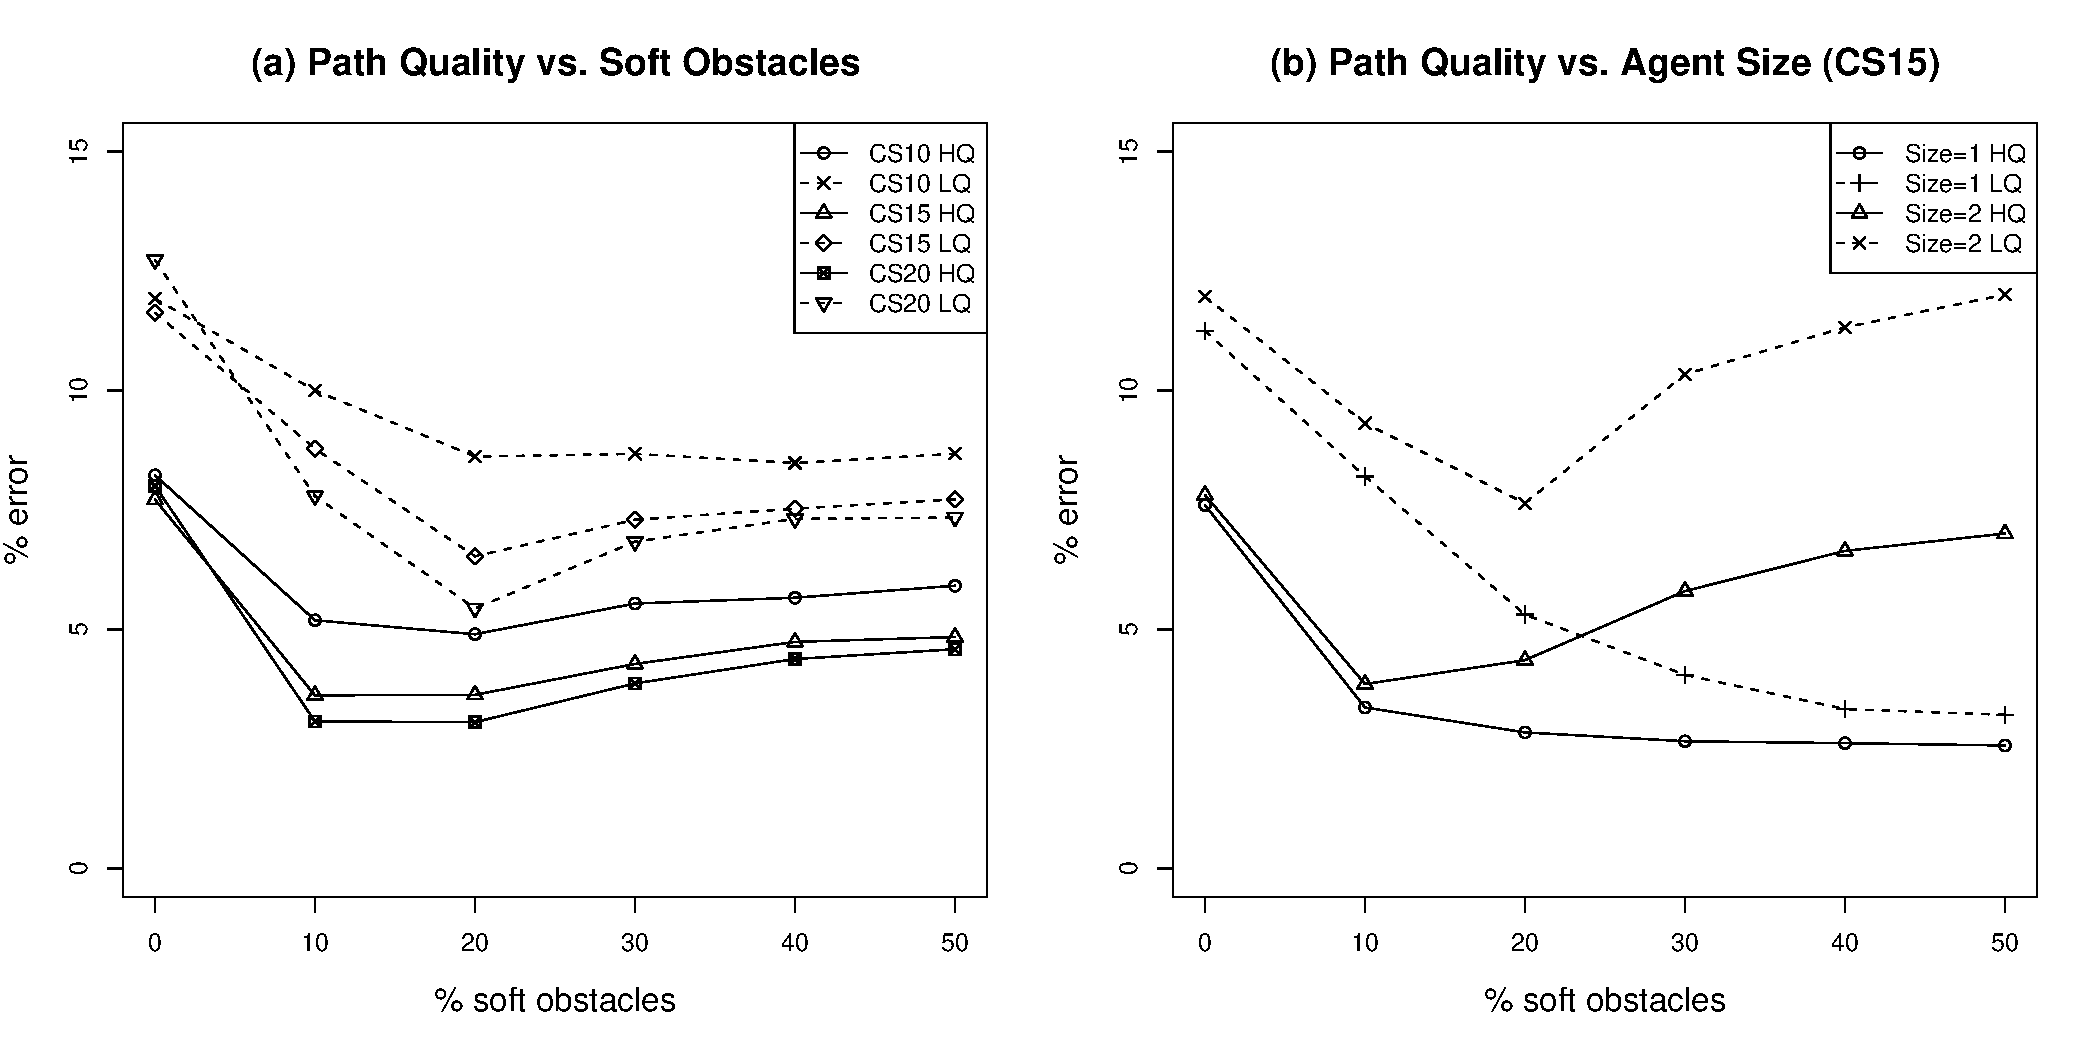
\includegraphics[scale=0.25, trim = 20mm 17mm 20mm 5mm]{diagrams/pathquality.pdf}
	\end{center}
	\label{aha-fig:pathquality}
	\vspace{-5pt}
\end{figure}
\par \indent
Figure \ref{aha-fig:pathquality}(a) shows the average performance of AHA* with respect to cluster size and soft obstacles.  
Notice that HQ graphs yield a very low error; in most cases between 3-6\%. 
Perhaps most encouraging however are the results for LQ abstractions, where in most cases AHA* performs within 6-10\% of optimal. 
The highest observed error in both cases occurs on SO 0\% and is due to our inter-edge placement strategy.
In all situations the pair of nodes with maximal clearance in an entrance, which we choose as our transition point, tends to be towards the beginning of the entrance area which is not an optimal placement.
On maps that produce low-complexity clusters of predominately one terrain this results in long entrances that are poorly represented by the single inter-edge.
Increasing the amount of soft obstacles produces shorter entrances and generates more transition points leading to a significant reduction in error. 
It appears AHA* is so optimised for complex cases that it suffers some minor performance degredation on simpler problems. 
\par \indent
Interestingly, the error associated with both HQ and LQ abstractions reaches a minimum on SO 20\% before gradually increasing toward SO 50\%. 
To better understand this phenomenon we present in Figure \ref{aha-fig:pathquality}(b) the performance of both small and large agents on HQ and LQ graphs using a fixed cluster-size of 15.
Notice that the performance of small agents continues to improve beyond SO 20\% while large agents begin to degrade.
The observed rise in error stems from the decreasing size of entrances on the problem sets featuring denser clusters. 
As previously shown in Figure \ref{aha-fig:graphsize}, maps with more soft obstacles result in a greater number of smaller entrances. 
This situation is beneficial for smaller agents (there are more transitions to choose from) but is disadvantageous for larger agents.
As the average entrance size shrinks fewer inter-edges exist with clearance $>$ 1 and the location of such edges along the border area between clusters may be quite varied; sometimes we find an entrance toward the beginning of the border area, other times in the middle and sometimes toward the end.
Consequently, cluster traversal by large agents is often not in a straight line; the abstract paths produced frequently feature a zig-zagging effect that is responsible for the observed error and is most pronounced on SO 50\%.
\begin{figure}[htbp]
	\vspace{-12pt}
	\caption{\small{\emph{AHA* total search effort (nodes expanded).}}}
	\begin{center}
		       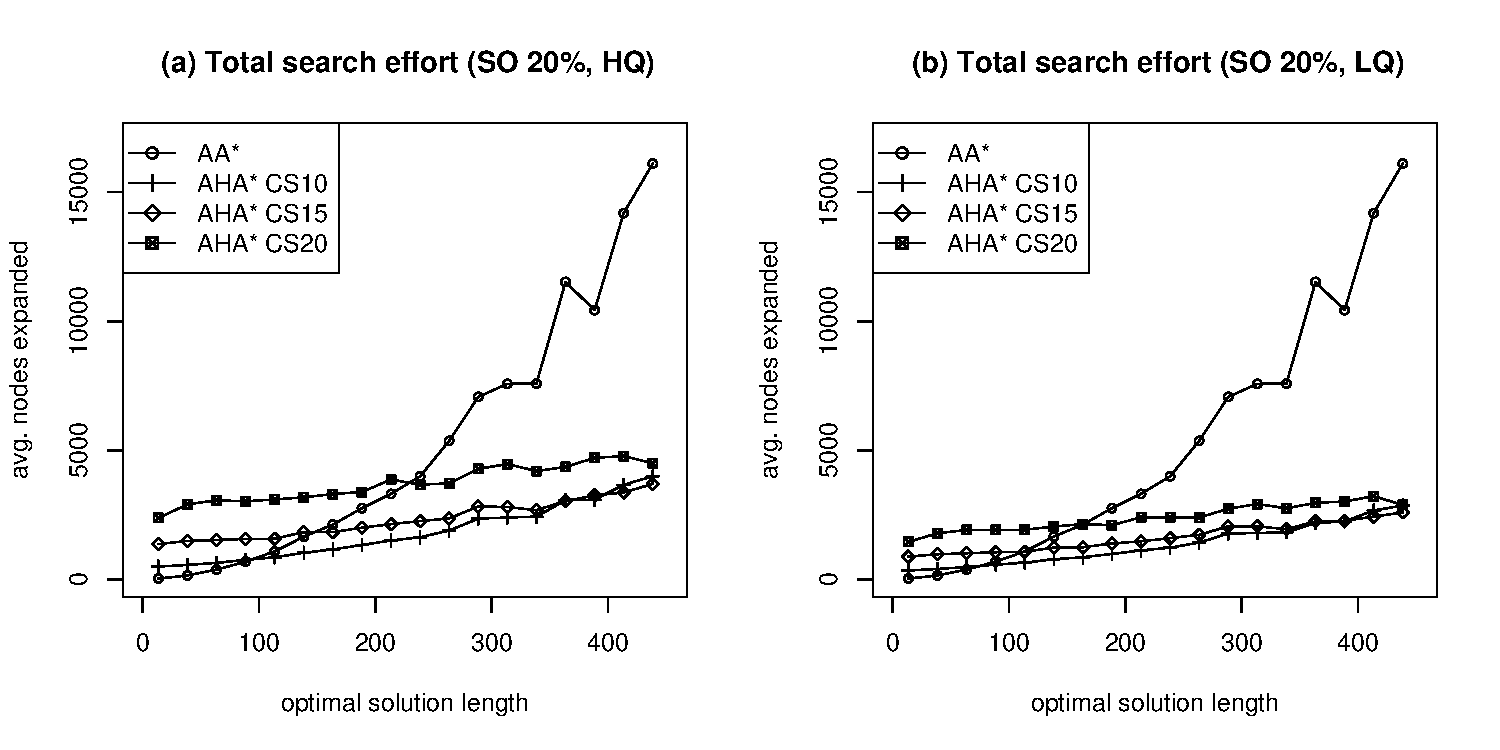
\includegraphics[scale=0.35, trim = 20mm 17mm 20mm 5mm]{diagrams/searcheffort.pdf}
	\end{center}
	\label{aha-fig:searcheffort}
	\vspace{-5pt}
\end{figure}
%\input setable.tex
\par \indent
Finally, we turn our attention to Figure \ref{aha-fig:searcheffort} where we evaluate AHA* using a search effort metric.
Here we contrast the total number of nodes expanded by AHA* (during insertion, hierarchical search and refinement phases) with AA* on both HQ and LQ graphs.
We focus on the SO 20\% problem set in order to analyse the effect on search effort as path length increases but note that similar trends hold for the other problem sets.
\par \indent
Looking at Figure \ref{aha-fig:searcheffort}(a) we observe that agents using HQ graphs featuring large cluster-sizes are disadvantaged in this test. 
The insertion effort required to connect start and goal to each abstract node in their local clusters heavily dominates the total effort causing AHA* CS20 to trail AA* for problems up to length 250.
We can see the gap between CS20 and the smaller cluster sizes decrease as problem size grows but our benchmark set of experiments are not hard enough for such coarse-grain map decompositions to be advantageous. 
By comparison, in Figure \ref{aha-fig:searcheffort}(b) we see that the difference is less pronounced using LQ graphs (there are less abstract nodes per cluster) however it appears CS10 or CS15 are more suitable choices for problems up to our maximum length, 450.
